\section{Measuring already deployed fiber}

Most of the methods described in section \ref{sec:calib_proc} require making a
measurement of 1-PPS signals produced by WR Devices. It's fairly easy to compare
them when you have a roll of fiber and the devices being calibrated lying on a
desk in the laboratory. However, sometimes the fiber infrastructure which
will be used in a WR network is already installed. WR Devices can still be
collected in a lab for calibration, but measuring the $\alpha$ parameter of a
buried fiber is not as straightforward as in section \ref{subsec:fiasym}. This
section proposes a way of measuring 1-PPS skew when the fiber cable is
already installed and you don't have both ends next to each other. The
measurements made this way can be used as a substitute for the simple
oscilloscope measurements in section \ref{sec:calib_proc}.

\subsection{Measurement with a loop-back fiber}
\label{subsec:loopback}
This method is based on a fiber delay calibration procedure used in the CERN
Neutrinos to Gran Sasso project \cite{cngs}. It requires:
\begin{itemize}
	\item an additional fiber which will be used to transmit the 1-PPS signal
		produced by a distant WR Device to the place where it can be compared
		locally with the other WR Device using an oscilloscope
	\item two oscilloscope cables of the same type - having equal latency or a
    known latency difference which can be taken into account and compensated
	\item one pair of optical transmitter and receiver which will be used to
		convert the 1-PPS electric signal into a light impulse sent through the
		loop-back fiber. The transmitter and receiver must have constant
		transmission/reception delays that don't vary on each power cycle.
\end{itemize}

\begin{figure}[ht]
	\begin{center}
	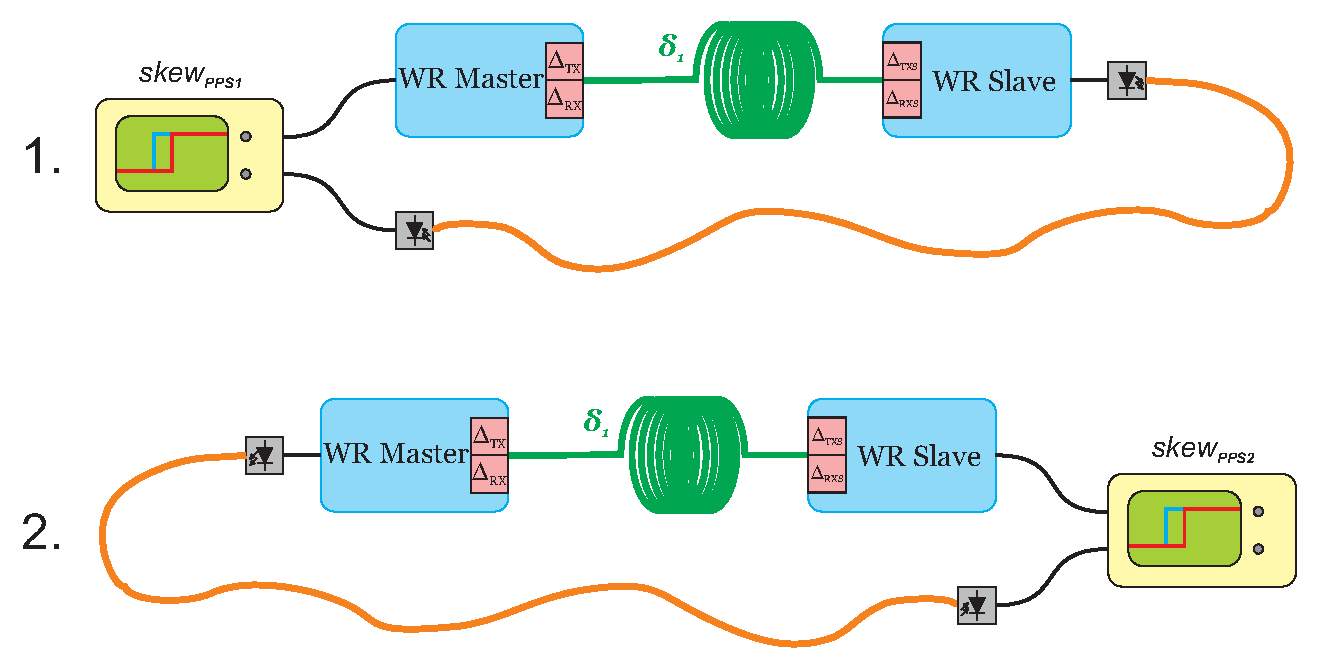
\includegraphics[width=.8\textwidth]{calibration/loopback_fibre.pdf}
	\caption{Measuring 1-PPS offset using a loop-back fiber}
	\label{fig:loopback}
	\end{center}
\end{figure}

Measurement procedure:
\begin{enumerate}
	\item When a link is established between the WR Master and the WR Slave,
		connect the optical transmitter to the 1-PPS signal produced by the WR Slave
		and the loop-back fiber. On the other side of the fiber connect the optical
		receiver (fig.\ref{fig:loopback}, step 1).
	\item Measure the 1-PPS skew ($skew_{PPS1}$) between the Slave (1-PPS
		transmitted through the loop-back fiber) and the Master (1-PPS directly from
		the node) using an oscilloscope.
	\item Swap the optical transmitter and receiver so that you'll now transfer
		the 1-PPS signal generated from the WR Master using the same loop-back fiber
		to the WR Slave side (fig.\ref{fig:loopback}, step 2).
	\item Do the same 1-PPS skew measurement between the Slave and Master, but
		this time on the WR Slave side (the 1-PPS comes directly from the WR Slave
		node and the one from the WR Master is transmitted through the loop-back
		fiber). This way you will obtain the value $skew_{PPS2}$.
	\item Calculate the actual skew between the WR Master and WR Slave using the
		equation:
	\begin{equation}
	skew_{PPS} = \frac{1}{2} (skew_{PPS1} + skew_{PPS2})
	\end{equation}
\end{enumerate}

The skew value calculated that way can be used in any equation from section
\ref{sec:calib_proc}. However, please remember that you will also need the
latency of the fiber ($\delta_1$ in figure \ref{fig:loopback}). That means, you
would have to start the calibration with two WR Devices on your desk, connected
with a short (few meters long) link (procedure \ref{subsec:refiber}) and later
use these two WR Devices with the already-installed link.
